%%%%%%%%%%%%%%%%%%%%%%%%%%%%%%%%%%%%%%%%%%%%%%%%%%%%%%%%%%%%%%%%%%%%%%%%%%%%%
\chapter{Practical Part}\label{chap:practicalPart}
%%%%%%%%%%%%%%%%%%%%%%%%%%%%%%%%%%%%%%%%%%%%%%%%%%%%%%%%%%%%%%%%%%%%%%%%%%%%%
\chapterstart

The practical part of this work is made up of three parts: the use case, a risk assessment and an example solution based on what was learned from the risk assessment. In the first part a use case is described. The use case tries to picture a typical scenario that requires thoughtful consideration of authentication and authorization technologies depending on the requirements of the use case. Based on the uses case a small risk assessment is done. This risk assessment should help to choose an appropriate level of assurance for identity proofing, authentication and federation. Based on this risk assessment a small application is implemented. The solution represents a federate single-sign on solution which uses modern open source authentication and authorization protocols. This procedure should help developers to choose appropriate authentication and authorization methods for a particular use case. The goal is to balance usability and security. 
\section{Use Case}
This use case is entirely fictional but allows the reader to get a better understanding of the circumstances a that led to the design of a federated authentication solution. 

The use case features a medium to large company with up to 1000 employees. The mission of the company is to provide a network and analyzing toolset which allows the customer of the product suite to improve security within his network and keep an overview of potential security risks. Previously the customers received monthly reports about their current state of the network. Each of the products and tools resulted in a separate report which was sent via E-Mail. To modernize the approach, the reports should be replaced by a modern single-page application that could be accessed by customers and by employees for administrative reasons. In this example, we call the solution 'Security Assessment Portal.' The Security Assessment Portal should give the customers an overview of current products and the performance of the network an example of the suit could be E-Mail-filtering.  

The company already has a particular set of internal applications that are used by the employees within the company network. The company internally uses active directory for authorization on local machines. All applications until now are accessible within the companies network and use windows authentication. The application should be accessible by employees as well as customers whereas customers should not receive access to the company network. The data of the customers are sensible and therefore worth protecting. Because of the highly sensible data, certain customer do not need which to authenticate with an external provider. The application should be hosted within the company a solution for customers to access the application from outside is needed. The company needs an authentication solution that meets all the outlined requirements while balancing usability and security. 


\section{Risk Assessment}

Risk Assessment is one of the essential elements when it comes to managing risks of an organization. The aim of risk assessment is it to identify, estimate, and prioritize risk to operations, assets, individuals, other organizations from the operations and use of the information system. The risks assessment should help to make decisions on how to respond to certain risk. The steps to a risk assessment are identifying potential threats, internal and external vulnerabilities, the impact to organizations given the potential for threats exploiting vulnerabilities and the likelihood of that harm to occur. There are three tiers according to (\cite{NIST:2012:GCRA}, p.1) in risk management:

\begin{itemize}
	\item Tier 1 - organizational level
	\item Tier 2 - mission/business process level
	\item Tier 3 - information system level
\end{itemize}

The first two Tiers are focusing on risks related to organizational governance and management activities, mission/business processes, enterprise architecture or the funding of information security programs. The third Tier focuses more on how to implement a risk management framework successfully [cf. (\cite{NIST:2012:GCRA}, p.1)]. 

The result of the risk assessment should state which assurance levels are appropriate. Identity proofing assurance level describes the robustness of the process to determine the identity of an individual and should help to avoid identity proofing errors. To determine the robustness of the authentication process and the binding of an authenticator and a specific individual's identifier the authentication assurance level is used. Furthermore choosing an appropriate authentication assurance level should help to avoid authentication errors. The last one of the assurance level is the federated assurance level which is optional since not all identity systems need a federated identity solution. The federated assurance level determines the robustness of the assertion protocol the federation uses to communicate authentication and attribute information and should help to avoid federation errors. All of the assurance levels a described in more detail in the sections \ref{identityProofing} Identity Proofing, \ref{authentication} Authentication and  \ref{assertion} Assertion [cf. (\cite{NIST:2017:DIG}, p.19)]. 

To determine assurance levels the potential risk and the measures to minimize the impact of this risk are identified. Two factors are crucial for this task. The first factor is the potential harm or impact, and the second the likelihood of such harm or impact. \cite{Bolton:2003:EAuth}, pp.3 splits harm and impact into these categories:

\begin{itemize}
	\item Inconvenience, distress, or damage to standing or reputation
	\item Financial loss or agency liability
	\item Harm to agency programs or public interests
	\item Unauthorized release of sensitive information
	\item Personal safety
	\item Civil or criminal violations
\end{itemize}

Assurance levels are determined by assessing the potential impact of these categories. \cite{NIST:2004:FIOPS} defines three levels of potential impact concerning security objectives confidentiality, integrity and availability. Those levels of potential impacts can affect either the organization or individuals should there be a breach of security. The levels of impact defined by \cite{NIST:2004:FIOPS} are:

\begin{itemize}
	\item Low
	\item Moderate
	\item High
\end{itemize}


If the level is low  the loss of confidentiality, integrity or availability has a limited effect. This can mean for example minor damage to organizational assets, short-term inconvenience, short-term distress, short-term embarrassment, limited reveal of personal or sensitive information to unauthorized parties with minor impact, minor financial loss, risk of civil or criminal violation which would not ordinary be subject to enforcement efforts, minor harm to individuals or the capability of the company to fulfill their mission is degraded. If the level of impact is moderate the effects of loss of confidentiality, integrity or availability are serious. Impacts can be significant damage to organizational assets, significant financial loss, serious short-term or limited longterm inconvenience,  serious short-term or limited longterm distress,  serious short-term or limited longterm damage to standing reputation, release of personal or sensitive information to unauthorized parties with moderate impact, risk of civil or criminal violations which may be subject to enforcement efforts, significant harm to individuals or significant degradation of mission fulfillment. The last level of potential impact is hight, meaning that the effects can be severe or catastrophic. This means for example major damage to organizational assets, major financial lost, severe or serious long-term inconvenience, severe or serious long-term distress, severe or serious long-term damage to standing reputation, release of personal or sensitive information to unauthorized parties with high impact, risk of civil or criminal violation with special importance to enforcement programs, harm to individuals involving loss of life or serious life threatening injuries and loss of capability to fulfill the mission [cf. (\cite{NIST:2004:FIOPS}, pp.6), (\cite{NIST:2017:DIG}, pp.21)].


To determine the minimum LOA needed the results of the risk assessment. The risk assessment impact profile can then be compared to the impact profiles associated with each assurance level. The table \ref{tab:maxImpacts} 'Maximum Potential Impacts for each Assurance Level' can hep to determine the required assurance level by finding the lowest level whose impact profile meets or exceeds the potential impact for every category analyzed in the risk assessment [cf. (\cite{NIST:2017:DIG}, p.25)].

\begin{table}[h]
		\centering
			\begingroup
		\setlength{\tabcolsep}{10pt} % Default value: 6pt
		\renewcommand{\arraystretch}{1.5} % 
	\begin{tabular}{lccc}
		\hline
		\rowcolor[HTML]{656565} 
		{\color[HTML]{FFFFFF} }                                                                                                     & \multicolumn{3}{c}{\cellcolor[HTML]{656565}{\color[HTML]{FFFFFF} Assurance Level}}                  \\ \hline
		\multicolumn{1}{|c|}{\textbf{Impact Categories}}                                                                            & \multicolumn{1}{c|}{\textbf{1}} & \multicolumn{1}{c|}{\textbf{2}} & \multicolumn{1}{c|}{\textbf{3}} \\ \hline
		\multicolumn{1}{|l|}{\begin{tabular}[c]{@{}l@{}}Inconvenience, distress or damage to\\ standing or reputation\end{tabular}} & \multicolumn{1}{c|}{Low}        & \multicolumn{1}{c|}{Mod}        & \multicolumn{1}{c|}{High}       \\ \hline
		\multicolumn{1}{|l|}{Financial loss or agency liability}                                                                    & \multicolumn{1}{c|}{Low}        & \multicolumn{1}{c|}{Mod}        & \multicolumn{1}{c|}{High}       \\ \hline
		\multicolumn{1}{|l|}{Harm to agency programs or public intrests}                                                            & \multicolumn{1}{c|}{N/A}        & \multicolumn{1}{c|}{Low/Mod}    & \multicolumn{1}{c|}{High}       \\ \hline
		\multicolumn{1}{|l|}{Unauthorized release of sensitive information}                                                         & \multicolumn{1}{c|}{N/A}        & \multicolumn{1}{c|}{Low/Mod}    & \multicolumn{1}{c|}{High}       \\ \hline
		\multicolumn{1}{|l|}{Personal safty}                                                                                        & \multicolumn{1}{c|}{N/A}        & \multicolumn{1}{c|}{Low}        & \multicolumn{1}{c|}{Mod/High}   \\ \hline
		\multicolumn{1}{|l|}{Civil or criminal violation}                                                                           & \multicolumn{1}{c|}{N/A}        & \multicolumn{1}{c|}{Low/Mod}    & \multicolumn{1}{c|}{High}       \\ \hline
	\end{tabular}
\endgroup
	\caption{Maximum Potential Impacts for Each Assurance Level (\cite{NIST:2017:DIG}, p.25)} \label{tab:maxImpacts}
\end{table}

When analyzing the risk it should be considered that there could be more then one error and multiple parties could be involved in the process. Furthermore the potential impacts description often include relative terms like 'minor' and 'serious' which meaning will depend on the context. Over time and with experience the meaning of these relative terms becomes more definite [cf. (\cite{NIST:2017:DIG}, p.26)].
 
One of the most useful documents is NIST's 'Guide for Conducting Security Risk assessment'. The guide follows activities related to NIST'S guide of 'Risk Management Framework' which can be either applied to new or legacy information systems. Typically a risk assessment is a very complex task that takes a lot of time an many external sources to be representative, like for example expert opinions. If put together correctly one should end up with a Risk Management Framework (RMF). A RMF provides a process that integrates security and risk management activities into the system development life cycle. The system can be applied to both new and legacy systems. \cite{NIST:2018:RMF} defines 6 Steps in this RMF. The steps include the categorization of information system, selection of baseline security controls, implementation of security controls, assessment of the security controls, authorize information system operation based on the determination of risk and monitoring security controls. Many industrial standard risk assessment methods across a wide array of fields and industries are based on these guides.  In this practical part an initial risk assessment is done which should provide a general feeling on how to to a risk assessment. The guide to success of a real life risk assessment is documentation, review and improvement.  However since a full RMF is out of the scope a scaled down version that is specific to digital identity risk management is conducted  (\cite{NIST:2018:RMF}].


To prepare for a risk assessment, it helps to identify the purpose, scope, assumptions, and constraints beforehand. The purpose of this risk assessment is to make authorization-related decisions and conducting an initial assessment to identify potential threats, internal and external vulnerabilities which impact the organizations. The scope addresses the 3 Tier -  information system level with focal point on the risk assessment of a single sign-on federation system. Furthermore, the scope is defined by the result expected from the risk assessment. In this risk assessment, the result should be an authentication and authorization solution for a specific use case. The assessment result should usually be reevaluated after the initial draft. [cf. (\cite{NIST:2012:GCRA}, pp.24)].

Before starting with the risk assessment a risk model hat to be chosen for the risk assessment. The model can be translated into risk factors which then can be assessed, these risk factor consist of threat, vulnerability, impact, likelihood and predisposed conditions.  A threat is a ny circumstance with the potential to impact the organization. Threat events are caused by threat sources. Threat sources that should be considered in the model can address broad thread sources or very specific threat sources. Potential threat sources can be adversarial like Insider, Outsider, Trusted Insider Privileged Insider, Customer, Competitor. A thread source can also be accidental like User, Privileged User/Administrator or structural like IT-Equipment (Storage, Communication, Processing), Environmental(Temperature/Humidity, Power Supply) or Natural (Fire, Bombing, Earthquake, Sunspots). These potential sources can then cause threat events which can be expressed very general or can also be very specific.Which thread are considered depend highly on the company. A company might choose to only considered previous observed events or all possible events. Examples for potential threat sources are Cause integrity loss by injecting false but believable data into organizational information systems, Obtain unauthorized access, Obtain sensitive data/information from publicly accessible information systems, Cause disclosure of critical and/or sensitive information by authorized users, Conduct externally-based session hijacking, Conduct simple Denial of Service (DoS) attack, Craft phishing attacks and so on. The likelihood is a weighted risk factor based on the probability that a given threat is capable of exploring a given vulnerability. A vulnerability is a existing weakness in an information system, system security procedures, internal controls, or implementation that could be exploited by a threat source. Most vulnerabilities are caused by security controls that are not implemented or not implemented correctly and still retain some weakness. Some recommended security controls are described in 'Recommended Security Controls for Federal Information Systems and Organizations'. The implementation of appropriate security controls is an important task that can have major impart on the operations and assests of a company. Security controls are used to protect the confidentiality integrity and availability of a system and its information. Examples are Identifier Management, Authenticator Management or Authenticator Feedback. Closely related to vulnerabilities are predisposed condition which is a condition within a company which affects the likelihood that threat events one initiated result in adverse impact on the organization like the involvement of PII. The consequences that an successfully exploited vulnerability by a threat source has is then described by the impact  [cf. (\cite{NIST:2012:GCRA}, pp17, pp35, pp70)].

Last but not least before stating a risk assessment based on a risk model an analytic approach and an assessment approach should be considered. The assessment approach can be quantitative, qualitative or semi-quantitative each of the factors including three assessment scales with corresponding different representations. A quantitative e assessment is based an the use of numbers whereas the qualitative assessment typically uses nonnumerical categories or levels like very low, low, moderate, high, very high. Finally, semi-quantitative assessment is a combination of a quantitative and a qualitative assessment using bins, scales or representative numbers which meaning ar not maintained in other contexts. For low impact information systems, the qualitative values ares used while for moderate-and hight-impact systems, the most granular semi-quantitative values are used. The analysis approach is either threat-oriented, asset/impact-oriented or vulnerability-oriented. The analysis approach basically lets one choose the starting point of the risk assessment. The risk assessment starting point van be either based on existing vulnerabilities or assets in the company or possible threats  [cf. (\cite{NIST:2012:GCRA}, pp17)].

Based on this knowledge a view examples considering the use case above where conducted. The following steps where followed based on the descriptions above Identify Threat, Identify Vulnerability, Current Controls, Likelihood of Impact, Effect of Impact and Risk Determination. The Likelihood of Impact can be assigned a value from low to high whereas high means it is very likely that a vulnerability is exploited by a threat. The lowest value of Likelihood of Impact is 0.1 and the highest is 1. The Effect of the Impact is assigned a value between 0 to 100. A low Effect of Impact means that the consequences are low and hight Effect of Impact means that the consequences are severe. To determine to overall risk of a threat the Likelihood is multiplied with the Impact (Likelihood x Impact) resulting in the risk levels:

\begin{itemize}
	\item Low =     0-33
	\item Medium = 34-66
	\item High =   67-100
\end{itemize}

Since this analysis is about identity proofing, authentication and federation errors a few threats  where chosen to be analyzed with the risk assessment to be analyzed. It should be noted that this does not represent a complete risk assessment since there are more factors to be possible considered. The risk analyses sees outsiders which want to harm the company and users as potential threat sources. 

\paragraph{Identity Proofing Risk 1}

\begin{enumerate}
	\item Technical Threat : An attacker successfully proofs as someone else
	\item Vulnerability :
	\item Current Controls : 
	\item Likelihood :
	\item Impact :
	\item \textbf{Risk Determination} : 
\end{enumerate}

\paragraph{Identity Proofing Risk 2}
\begin{enumerate}
	\item Technical Threat : Collecting and securely storing more information about a person than is required to successfully provide the digital service
	\item Vulnerability :
	\item Current Controls : 
	\item Likelihood :
	\item Impact :
	\item \textbf{Risk Determination} : 
\end{enumerate}

\paragraph{Identity Proofing Risk 3}
\begin{enumerate}
	\item Technical Threat : Number of retries allowed (brute force)
	\item Vulnerability :
	\item Current Controls : 
	\item Likelihood :
	\item Impact :
	\item \textbf{Risk Determination} : 
\end{enumerate}


\paragraph{Authentication Risk 1}
\begin{enumerate}
	\item Technical Threat : False claimant using a credential that is not rightfully theirs
	\item Vulnerability :
	\item Current Controls : 
	\item Likelihood :
	\item Impact :
	\item \textbf{Risk Determination} : 
\end{enumerate}

\paragraph{Authentication Risk 2}
\begin{enumerate}
	\item Technical Threat : Account is compromised and user is using same identifier and authenticator for other accounts
	\item Vulnerability :
	\item Current Controls : 
	\item Likelihood :
	\item Impact :
	\item \textbf{Risk Determination} : 
\end{enumerate}

\paragraph{Authentication Risk 3}
\begin{enumerate}
	\item Technical Threat : Feedback from application allows unauthorized user to compromise authentication mechanism
	\item Vulnerability :
	\item Current Controls : 
	\item Likelihood :
	\item Impact :
	\item \textbf{Risk Determination} : 
\end{enumerate}

\paragraph{Federation Risk 1 }
\begin{enumerate}
	\item Technical Threat : An identity assertion is compromised
	\item Vulnerability :
	\item Current Controls : 
	\item Likelihood :
	\item Impact :
	\item \textbf{Risk Determination} : 
\end{enumerate}

\paragraph{Federation Risk 2}
\begin{enumerate}
	\item Technical Threat : Transaction involving third party not over protected channel
	\item Vulnerability :
	\item Current Controls : 
	\item Likelihood :
	\item Impact :
	\item \textbf{Risk Determination} : 
\end{enumerate}




Modern digital services often combine identity proofing, authentication and federation requirements in one single bundle. It is better to look at each of this components separately to delivery the best identity service [cf. (\cite{NIST:2017:DIG}), (\cite{NIST:2018:RMF}].

TODO: Your text here ...


\section{Solution}
The \cite{Sakimura:2014:OpenIDConnect} explains that modern applications have different requirements than their predecessor due to new distributed architectures that allow enterprises to be more flexible. Cloud or Microservice architectures require different interactions between applications as the \ref{fig:architecture-identityserver} below show the most common interactions for modern applications.

\begin{figure}[h]
	\centering
	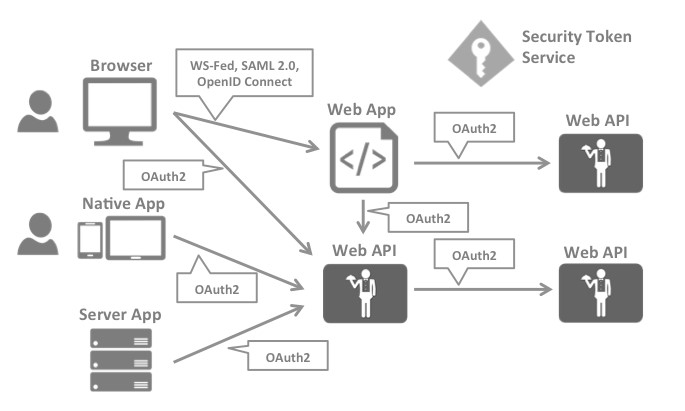
\includegraphics[width=0.9\linewidth]{images/architecture-identityserver}
	\caption[Architecture IdentityServer4]{Architecture IdentityServer4}
	\caption{Architecture IdentityServer4}
	\label{fig:architecture-identityserver}
\end{figure}





For example, a browser might call a Web App, and a Web App calls a Web API or perhaps a Native App calls a Web API, which is calling another Web API. Each application has to implement security functions to maintain a secure flow throughout these interactions, Implementing this security features for each involved application leads to a lot of duplicated code and inconsistencies. A different approach to implement security throughout these flows is using a token service. A token service brings the benefit of being able to encapsulate these security functions. Security functions can be updated and hosted at a single point which prevents duplicated functions across applications and security flaws [cf. (\cite{Sakimura:2014:OpenIDConnect})].

Identity Server4 is an ASP.NET framework that uses the specifics of OpenID Connect and OAuth 2.0 to enable Authentication and Authorization related features. Features include Authentication as a Service, which provides a centralized login logic for all applications, Single sign-on, Access Control for APIs and Federation Gateway. The Identity Server 4 will be used as a Token Server in the practical part [cf. (\cite{Brock:2018:ID4})]

The project illustrating the use of Identity Server and the benefits of OpenID Connect an OAuth is a Visual Studio Project mostly written in C\# and Typescript. The project example for Identity Server includes four different projects:

\begin{itemize}
	\item Identity Server - The Identity Server is a ASP.NET Core Project with basic Implementation of an Identity Server which serves as a Token Server. 
	\item ProjectApiNetCore - This application is a ASP.NET Core 2.0 API Application with basic API that returns the users Claims if he is authenticated.
	\item Angular Client - The Angular Client is a ASP.NET Core MVC Angular Project used as a Client that can be accessed by an End-User who can authenticate with the Identity Server and requests protected resources of the API ProjectApiNetCore.This project uses the Implicit Code Flow. 
	\item MVC Client - The MVC Client is a ASP.NET Core MVC Project used as a Client that can be accessed by an End-User and can authenticate with the Identity Server and requests protected resources of the API ProjectApiNetCore. This project uses the Hybrid Code Flow. 
\end{itemize}



\paragraph{Identity Server}

This project is using the IdentityServer4 library by Brock Allen and Dominick Baier. The Project works as a Token Server which means that the Identity Server Project is responsible for authentication the user, managing the identities and provide and approve tokens. Furthermore, the Identity Server implements different Authentication Flows.


\begin{figure}[h]
	\centering
	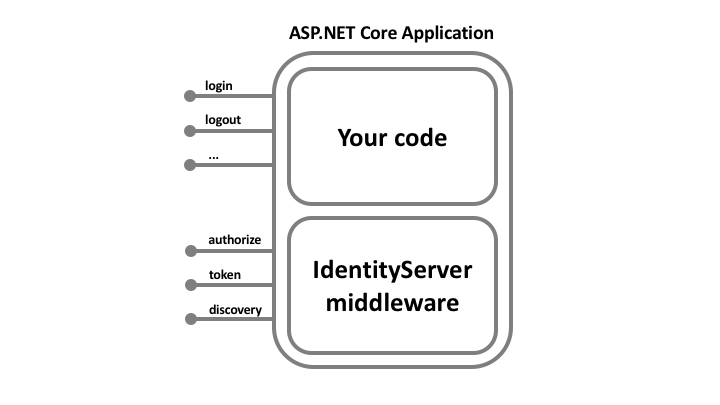
\includegraphics[width=0.8\linewidth]{images/middlewareIdentityServer}
	\caption{IdentityServer Middleware}
	\label{fig:middlewareidentityserver}
\end{figure}
 

IdentityServer4 adds endpoints of OAuth 2.0 and OpenID Connect to an arbitrary ASP.NET Core application as shown in \ref{fig:middlewareidentityserver}. The identity server can be as complex as the developer wants but \cite{Brock:2018:ID4} recommends to keep the attack surface as small as possible by just including authentication related UI only [cf. (\cite{Brock:2018:ID4})]. 


For the basic Setup, the Identity Server has to be added to the StartUp class and to ensure a secure communication a certificate has is created to sign the request. For the basic setup, Identity Server provides us with DeveloperSigningCredentials which provides a dummy certificate. In this example application, a real certificate is included. 

\begin{figure}[h]
	\centering
	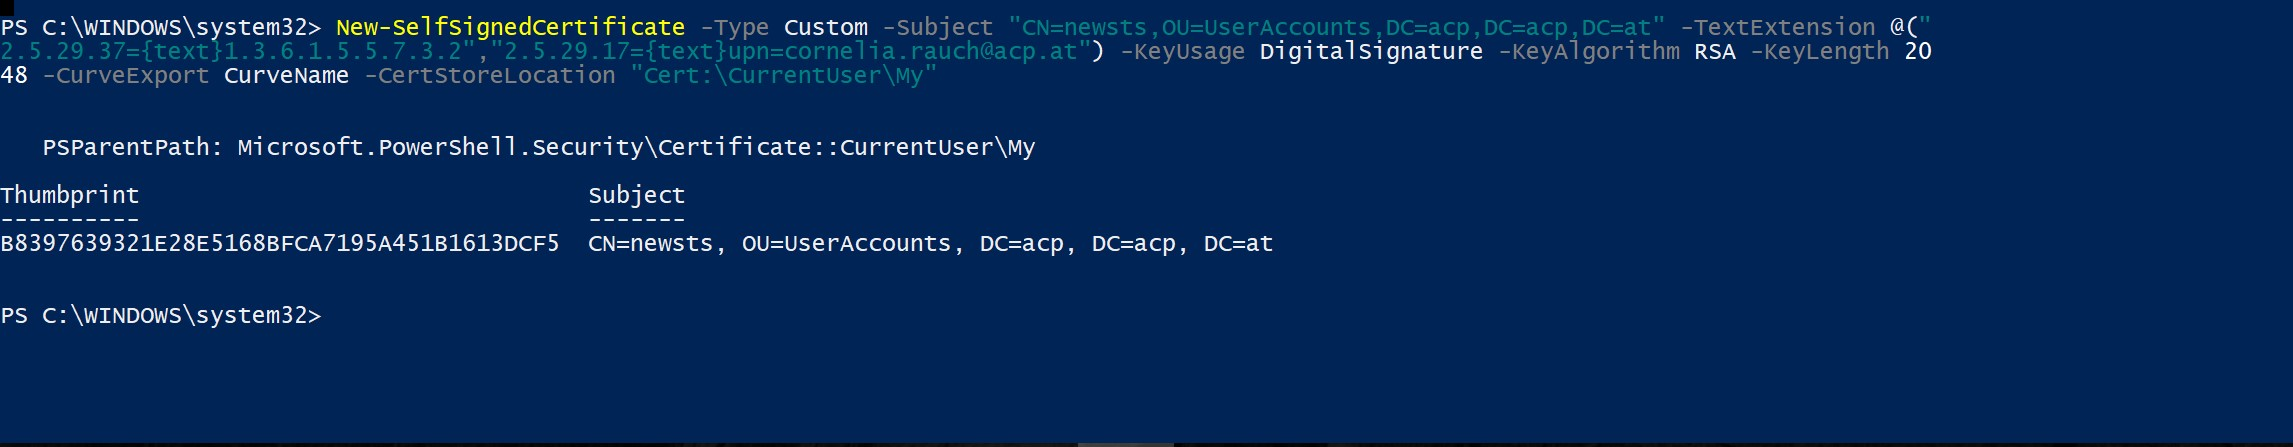
\includegraphics[width=0.8\linewidth]{images/self-signed-certicate}
	\caption{Self signed Certicate with Powershell}
	\label{fig:self-signed-certicate}
\end{figure}

The certificate used in this application was created with Powershell as shown in \ref{fig:self-signed-certicate}. The algorithm used in this certificate is RSA. Depending on the algorithm that is used in the certificate a similar hashing algorithm has to be used for the Client Secret.


The API Resources include the available APIs that can be called and included in the scope of a request. The Identity Resources are Resources that can be included in the returning id\_token. The Clients are the available Clients that can be configured and can use the Identity Server. Those Client Configurations indicate which Authorization Flow is used and how to retrieve id\_token, access\_token, and a possible refreh\_token. For simplifying reasons, Identity Server provides an in Memory User Storage which can be used for Testing reasons. Other ways to define Users are via .NET Core Identity or IdentityServer4 EntityFramework. For the purpose of this implementation this Test Users where included in the Identity Server application:
\begin{enumerate}
	\item User1:
	\begin{itemize}
		\item  Username: bob
		\item  Password: bob
	\end{itemize} 
	\item User2:
	\begin{itemize}
		\item  Username: alice
		\item  Password: alice
	\end{itemize} 
\end{enumerate}

After the basic setup of the Identity Server, it can be examined if the Identity Server is running correctly by calling the discovery document. The discovery document can be used by the Clients and APIs to retrieve necessary configuration data. The Identity Server has to run at local port 5000 and in the browser navigate to
\url{http://localhost:5000/.well-known/openid-configuration}.

\begin{figure}[h]
	\centering
	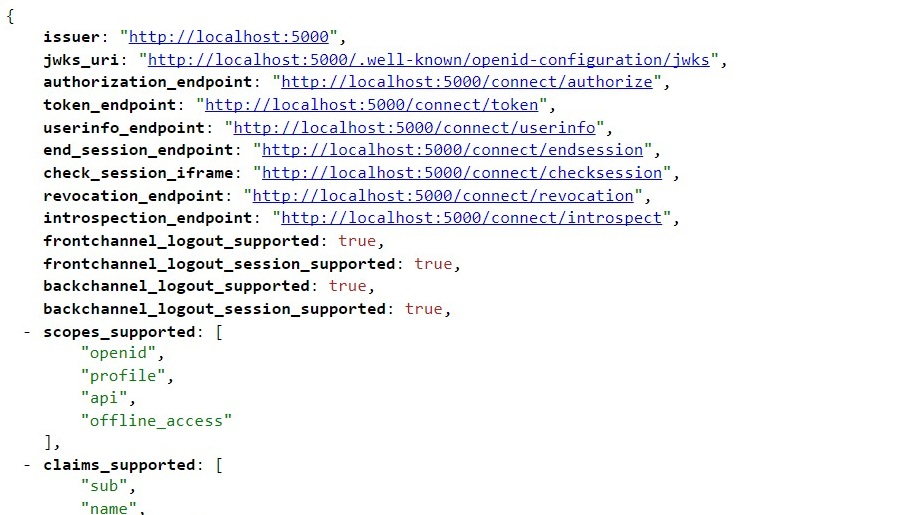
\includegraphics[width=0.8\linewidth]{images/openid-discovery-document}
	\caption{OpenID Discovery Document}
	\label{fig:openid-discovery-document}
\end{figure}
The discovery document is located at a well-known location and is containing key-value pairs as a JSON structure. The key-value pairs int he discovery document represent multiple endpoints that are used to authenticate a user including URIs of the authorization, token, userinfo, and public-keys endpoint. The use of a discovery document brings more flexibility to the protocol brings more flexibility. The application should have the discovery URL hard-coded in the application according to (\cite{Google:2018:IdentityPlatform}) the discovery document URL can then be used to fetch endpoints from the document and use them to for example send an authentication request [cf. (\cite{Google:2018:IdentityPlatform})].

The metadata that is seen in \ref{fig:openid-discovery-document} OpenID discovery document is a mixture of required elements with some recommended ones that are implemented by the identity server. The required elements are issuer, authorization\_endpoint, token\_endpoint, jwks\_uri, response\_types\_supported, subject\_types\_supported and id\_token\_signing\_alg\_supported. The issuer, in this case, is this Identity Servers address. The authorization\_endpoint is the URL OAuth 2.0 Authorization Endpoint. The user is redirected to the authorization server's authorization endpoint for authentication and authorization. The authentication request that is sent to the authorization server can have different request parameters. These request parameters are defined by OAuth 2.0 and additional request parameters defined by OpenID Connect. The token\_endpoint is the URL of the OAuth 2.0 Token Endpoint. The RP can request access or optionally refresh tokens from the token endpoint. The user\_endpoint can be used to request additional information concerning the user. The response\_types\_supported is important information about what kind of response is supported and ultimately what kind of authentication flow can be used based on that information like described in chapter \ref{chap:authenticationandauthorization} in Single-Sign on Federate Systems. The subject\_types\_supported is a list of subject identifier types. Moreover, last but not least id\_token\_signing\_alg\_supported is used to find out which JWS is signing algorithm is used to encode the ID token and get the claims of the JWT. The algorithm RS256 must be included [cf. (\cite{Sakimura:OIDCC}, (\cite{Sakimura:OIDCD}))].. 

\begin{figure}[h]
	\centering
	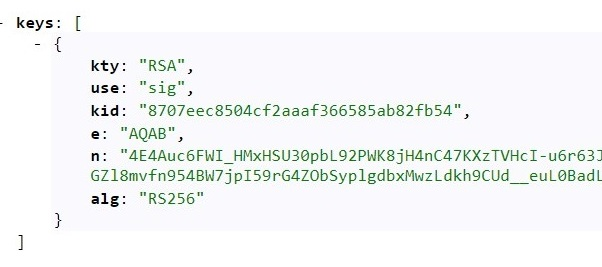
\includegraphics[width=0.7\linewidth]{images/jwkDiscovoryDocument}
	\caption{JWKS Endpint}
	\label{fig:jwkdiscovorydocument}
\end{figure}

The jwks\_endpoint is worth a closer look. JWKS SET is published to the JWKS endpoint. The keys shown in (\ref{fig:jwkdiscovorydocument} JWKS Endpoint) can be rolled over by periodically adding new keys to the JWK Set. This also indicates if the cryptographic algorithms are configured correctly. E.g. : The message is using the kid of signing key in the JOSE Header to indicate which key has to be used to validate the signature. The algorithm used by the signing party has to be supported by the recipient and can be either and Asymmetric Signature or a Symmetric Signature. 
When using RSA or ECDSA signatures, the alg Header Parameter has to be set to the correct algorithm, and the private key used to sign must be associated with the public key published by the sender. When using MAC-based signatures, the alg Header Parameter has to be set to the correct algorithm, and the MAC key is the octets of the UTF-8 representation of the client\_secret. MAC-based signatures cannot be used by public Clients because they cannot keep secrets.  All metadata types are listed in the specification of OpenID Discovery Document from \cite{Sakimura:OIDCD} [cf. (\cite{Sakimura:OIDCC}, (\cite{Sakimura:OIDCD}))]. 

After calling the OpenID discovery document and the JWKS endpoint, one can be ensured that the basic setup of the IdentityServer works. Next, a resource that is worth beeing protected by the Identity Server has to be created. 

\paragraph{ProjectApiNetCore}

This ProcjectApiNetcore is an ASP.NET Core application. This application represents the Resource Server and serves the Protected Resources. In this particular example, the API provides a list of Products the user bought from the company and the possibility to download the report that gives information about the current state of the product. The example API provides dummy data for the particular request. For easy testing of the API and designing the API, swagger.io is used. Furthermore, swagger.io (\url{https://swagger.io/}) gives a nice developer experience with an interactive API documentation. In addition, it is possible to generate code out of the swagger documentation for different programming languages with tools like NSwag (\url{https://github.com/RSuter/NSwag}).

\begin{figure}[h]
	\centering
	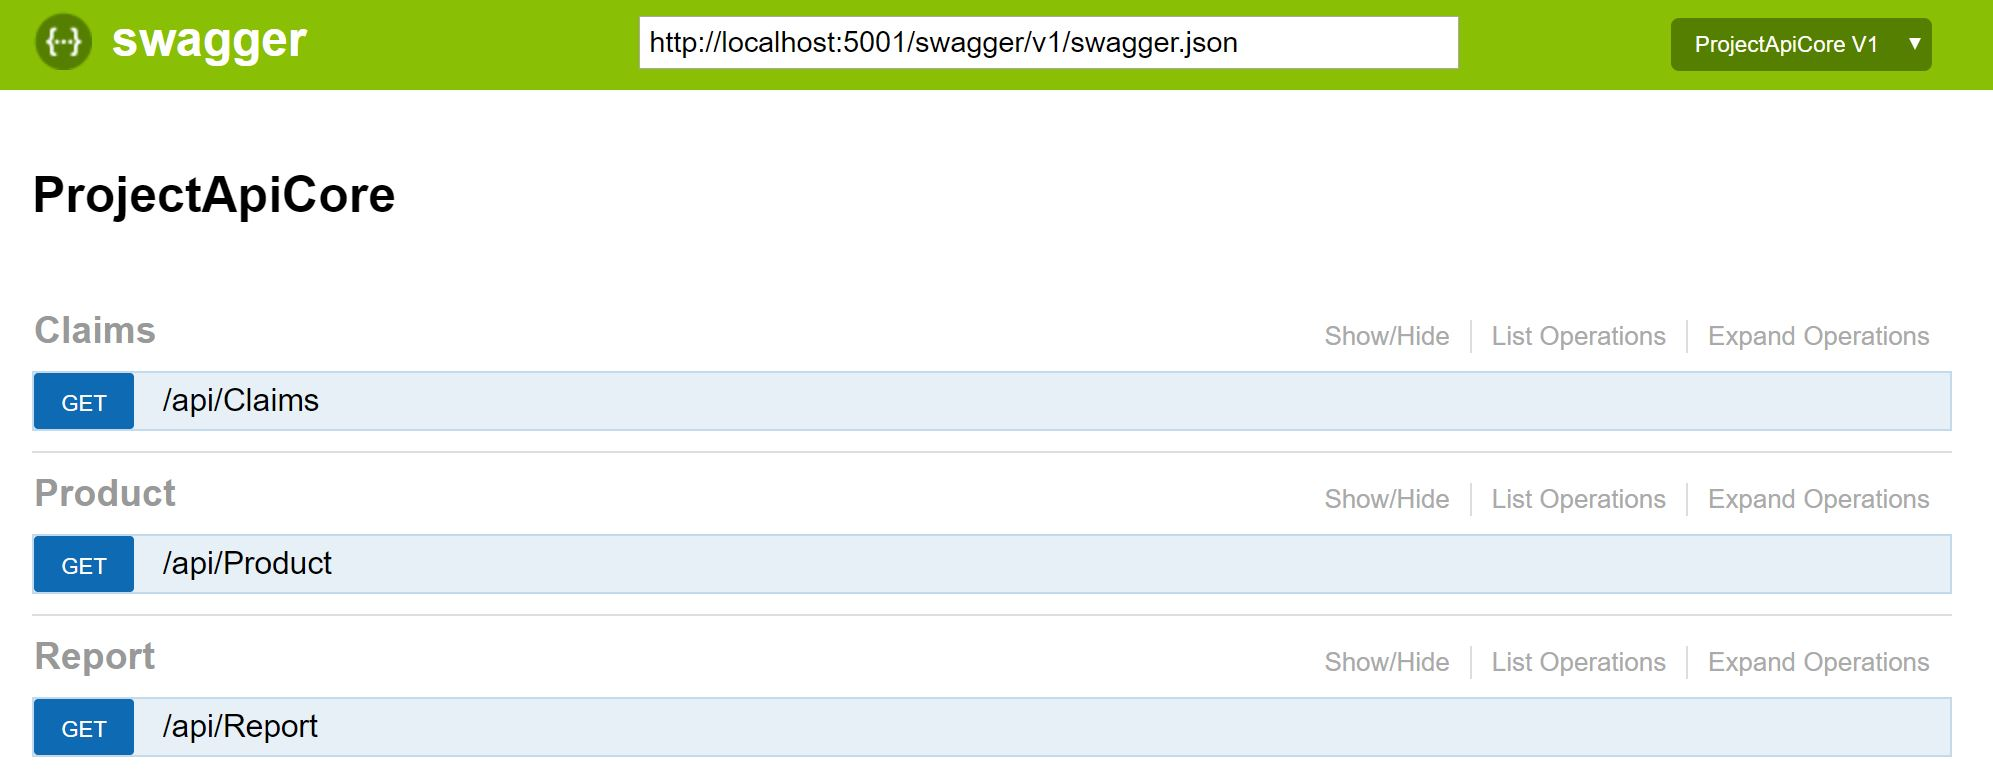
\includegraphics[width=0.7\linewidth]{images/apis}
	\caption{API documentation with Swagger}
	\label{fig:apis}
\end{figure}

All of the routes shown in \ref{fig:apis} API documentation with Swagger, are secured with the help of the IdentityServer4.AccessTokenValidation NuGet package. Each Controller gets an Authorize annotation. 
To configure the right authentication method, ASP.NET Core 2.0 offers the possibility to add the authentication to the pipeline with Dependency Injection via the method Configure Services in the Startup.class.
In the StartUp class of the API Project the AddAuthentication with the Value "JwtBearerDefaults.AuthenticationSchemeMakes "Bearer" the default authentication scheme “Bearer”. With the AddIdentityServerAuthentication it is defined which Token server can be used to validate the incoming token and make sure that this token is from a trusted issuer. It adds the Identity Server access token validation handler into DI and also it is checked if the token is valid to be used with this API (aka scope). Adding UseAuthentication to the Configure method int the Startup class adds the authentication middleware to the pipeline so authentication will be performed automatically on every call into the host.  Multiple authentication schemes can be used. A list of authentication schemes is then passed to the Authorize attribute separated with a comma. The default scheme results in the HttpContext.User property is set to that identity. After adding the Authentication logic to the API Project, the resources should be protected know. To check if the resources are protected the Swagger documentation can be used. Therefore one has to navigate to \url{http://localhost:5001/swagger/v1/swagger.json} and try out one of the methods shown in (\ref{fig:apis}) API Documentation with Swagger. This should result in a 401 Unauthorized HTTP response code.

 

TODO: Your text here...

\chapterend
